\chapter{Apprendimento Supervisionato}
\section{Dati}
Un insieme di record di dati $X \in X^k$, chiamati anche \textbf{esempi}, \textbf{istanze} o \textbf{casi} sono descritti da:
\begin{itemize}
  \item $k$ attributi (\textbf{Features}): $x = {x_1, x_2, \cdots, x_k}$.
  \item Una \textbf{classe}: ogni esempio è etichettato con una classe target predefinita $c \in C$.
\end{itemize}
L'obiettivo è imparare un modello di classificazione dai dati che possono essere usati per predire la classe di nuovi casi.

\section{Processo di Apprendimento Supervisionato}
Il processo è diviso in due step:
\begin{enumerate}
  \item Imparare un modello usando idati dell'allenamento.
  \item Testare il modello con dati mai usati per vederne l'\textbf{accuratezza}.
\end{enumerate}
\[
  \text{Accuratezza} = \frac{\text{Numero di classificazioni corrette}}{\text{Numero totali di casi}}
\]

\begin{figure}[!htb]
    \centering
    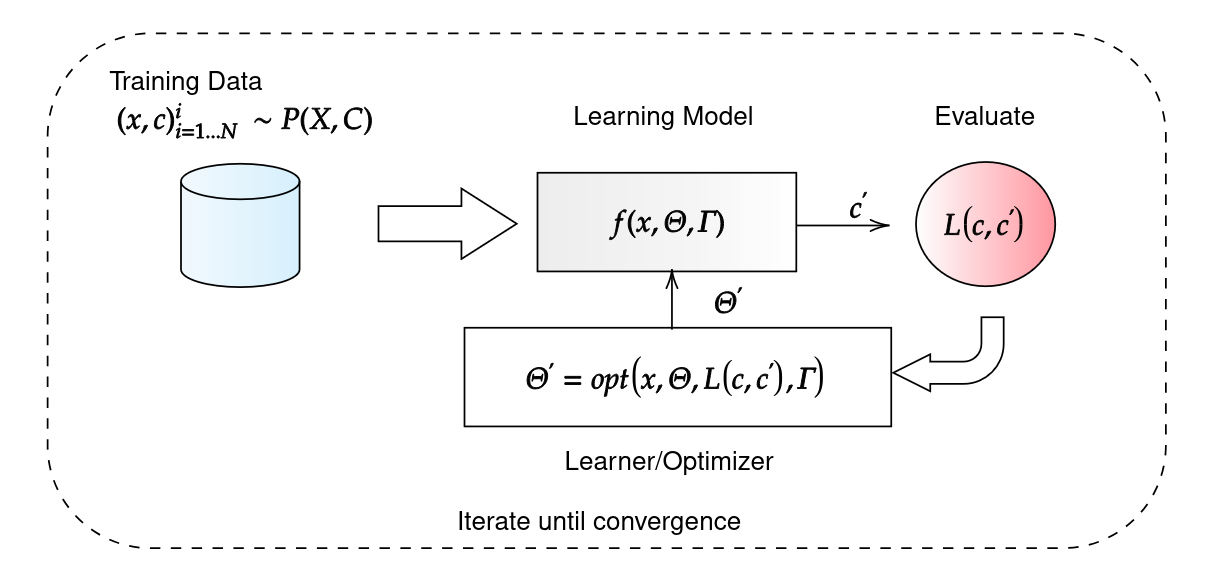
\includegraphics[width=0.5\linewidth]{Images/sup_learning/Training.png}
    \caption{Training pipeline.}
\end{figure}

\begin{figure}[!htb]
    \centering
    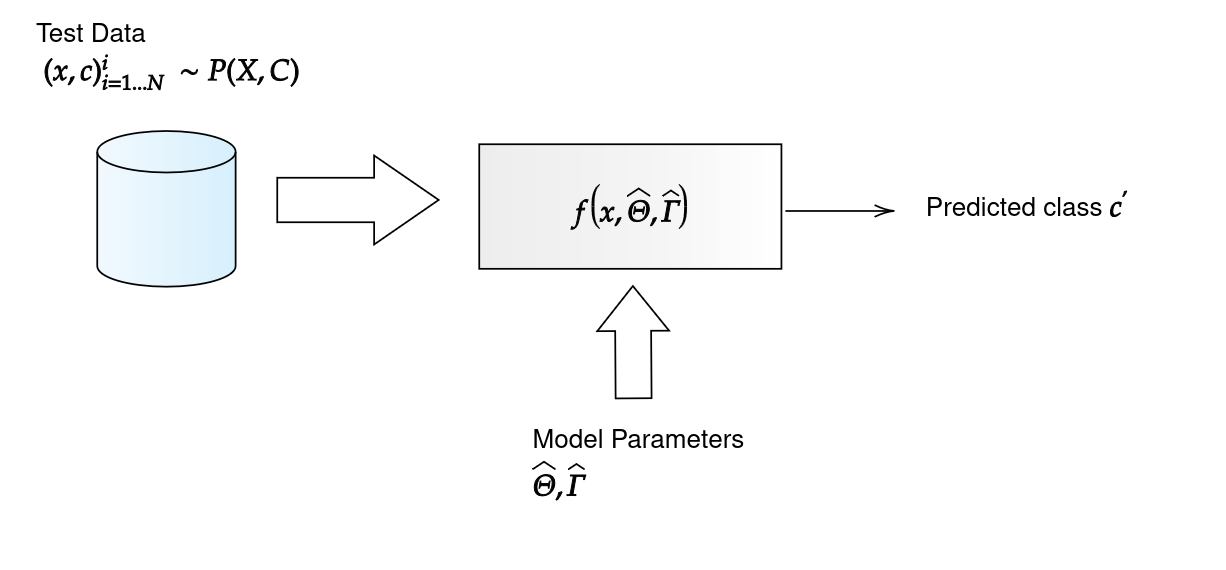
\includegraphics[width=0.5\linewidth]{Images/sup_learning/Inference.png}
    \caption{Inference pipeline.}
\end{figure}

\section{Apprendimento}
\begin{defn}[Apprendimento]
  Dati un dataset $D$, una classe compito $C$ e una funzione di prestazione $L$, si dice che un sistema informatico apprende il compito $C$ dai dati $D$ se,
  dopo aver osservato $D$, la prestazione misurata tramite $L$ migliora fino a raggiungere un livello superiore a quello di una scelta casuale.
\end{defn}

In altre parole, i dati aiutano il sistema a migliorare le proprie prestazioni rispetto all'assenza di apprendimento.

\begin{note}[Assunzione fondamentale i.i.d]
  L'apprendimento è possibile solo se il training e l'inferenza sono fatti usando dati dalla stessa distribuzione $x \sim P(X)$.
  Detto questo, i campioni usati sono indipendenti e identicamente distrbuiti (i.i.d), dal training all'inferenza.
\end{note}

\subsection{Misure di valutazione}
Oltre all'accuratezza, che abbiamo visto in precedenza, ci sono molti altri metodi per valutare:
\begin{itemize}
  \item \textbf{Efficenza:}
  \begin{itemize}
    \item Tempo usato per costruire il modello.
    \item Tempo per usare il modello.
  \end{itemize}
  \item \textbf{Robustezza:} gestire il rumore e valori mancanti.
  \item \textbf{Scalibilità:} efficenza in database basati su dischi.
  \item \textbf{Interpretabilità:} comprensibilità e approfondimenti forniti dal modello.
  \item \textbf{Compattezza del modello:} dimensione dell'albero o numero di regole.
\end{itemize}

\subsection{Modello di valutazione}
Un modello usato è l'\textbf{Holdout Set}, dove il dataset $D$ a dispozione viene diviso in due insiemi disgiunti:
\begin{itemize}
  \item \textbf{Insieme per il training}, $T_r$.
  \item \textbf{Insieme per l'inferenza}, $T_e$.
\end{itemize}

\begin{note}[Nota Bene]
  L'insieme di addestramento non deve essere utilizzato per i test e l'insieme di test non deve essere utilizzato per l'apprendimento.
  Un insieme di test non visto fornisce una stima imparziale dell'accuratezza.
\end{note}
Questo metodo è solitamente usato quando i dataset $D$ sono molto larghi.

\section{Iperparametri}
Tutti i classificatori presentano parametri aggiuntivi, denominati \textbf{iperparametri} e non vengono appresi, bensì selezionati in fase di progettazione prima dell'addestramento. \\
Diverse configurazioni degli iperparametri possono modificare in modo significativo le prestazioni del modello. \\
Viene usata un'ulteriore suddivisione del dataset $D$, utilizzata per la messa a punto degli iperparametri e per la selezione del modello migliore, chiamato \textbf{insieme di validazione}.

\newpage
\begin{ex}[Train-Validation-Test]
  \begin{itemize}
    \item Dato un dataset $D$, partizioniamo randomicamente i dati in un insieme di allenamento $T_r$, uno per la validazione $V$ e uno per il test $T_e$. Di solito con  60/20/20, 80/10/10 o simile.
    \item I modelli $M_i$ imparano su $T_r$ per ogni scelta dell'iperparametro $H_i$.
    \item L'errore di validazione $Val_i$ di ogni modello $M_i$ viene valutato sull'insieme $V$.
    \item Vengono selezionati gli iperparametri $H_*$ che presentano il valore più basso di $Val_i$ e il classificatore viene riaddestrato utilizzando tali iperparametri sull'insieme $T_r + V$, ottenendo un modello finale $M_*$.
    \item La capacità di generalizzazione viene stimata valutando l'errore o l'accuratezza di $M_*$ sui dati dell'insieme di test $T_e$.
  \end{itemize}
\end{ex}

\begin{ex}[k-fold Crossvalidation]
  Il metodo viene spesso utilizzato quando il dataset non è sufficientemente ampio da consentire di ottenere un test set consistente.
  \begin{itemize}
    \item Partizioniamo randomicamente un dataset $D$ in un insieme di $K$ blocchi $B_1, \cdots, B_k$.
    \item Per ogni fold di cross-validation $k = 1, \cdots, K$:
    \begin{itemize}
      \item Assegna $T_e = B_k$ e $T_r = D - {B_k}$ (i rimanenti $K-1$ blocchi).
      \item Impara il modello $M_k$ su $T_r$ e testalo su $B_k$.
    \end{itemize}
    \item Il processo produce $k$ accuratezze.
    \item La stima finale delle prestazioni del modello è la media delle $K$ accuratezze.
  \end{itemize}
\end{ex}

\section{Altre Misure di Classificazione}
L'accuratezza non è l'unica misura e in alcuni casi non è nemmeno utilizzabile. Per questo vengono usate anche misure:
\begin{itemize}
  \item \textbf{Precisione:} è il numero di esempi positivi classificati correttamente diviso per il numero totale
  di esempi classificati come positivi.
  \[
    p = \frac{TP}{TP + FP}
  \]
  \item \textbf{Recall:} è il numero di esempi positivi correttamente classificati diviso per il numero totale
  di esempi positivi effettivi nell'insieme di test.
  \[
    r = \frac{TP}{TP + FN}
  \]
\item \textbf{F1-score:} è la media armonica di precisione e recall. Dà maggior peso al valore più basso.
\[
  \frac{1}{F1} = \frac{1}{p} + \frac{1}{r}
\]
\end{itemize}

\begin{defn}[Cross-Entropy]
  La cross-entropy è una misura della teoria dell'informazione relativa alla codifica dei messaggi utilizzando il numero di bit.
  Valuta il numero medio di bit per scoprire un dato codificato da una distribuzione $Q$ mentre quello originale era $P$.
  \[
    \mathbb{E}_P[l_i] = \sum_x{P(x)\log_2{\frac{1}{Q(x)}}} = - \sum_x{P(x)\log_2{Q(x)}}
  \]
\end{defn}
